%CS-113 S19 HW-2
%Released: 15-February-2019
%Deadline: 26-February-2019 5.00 pm
%Authors: Muhammad Usaid, Shehryar Mughal, Mudasir Hanif Shaikh


\documentclass[addpoints]{exam}
% Header and footer.
\pagestyle{headandfoot}
\runningheadrule
\runningfootrule
\runningheader{Problems for Beginners}{Open Discrete Mathematics}{First Edition}
\runningfooter{}{Page \thepage\ of \numpages}{}
\firstpageheader{}{}{}
\usepackage{mathtools}
\usepackage{amsmath}

\newcommand*{\Perm}[2]{{}^{#1}\!P_{#2}}%
\newcommand*{\Comb}[2]{{}^{#1}C_{#2}}%

\DeclarePairedDelimiter\ceil{\lceil}{\rceil}
\DeclarePairedDelimiter\floor{\lfloor}{\rfloor}
\boxedpoints
\printanswers
\usepackage[table]{xcolor}
\usepackage{amsfonts,graphicx,amsmath,hyperref,amssymb}
\hypersetup{
    colorlinks=true,
    linkcolor=blue,
    urlcolor=cyan,
}




\begin{document}
	
\begin{titlepage}
	\begin{center}
		\vspace*{1cm}
		
		\textbf{\Huge OPEN DISCRETE MATHEMATICS}
		
		\vspace{4cm}
		
		\text{\huge Discrete Maths Problem Set with Solutions}
		
		\vspace{0.5cm}
		{\LARGE An Open Source Problem Set for Beginners}
		
		\vspace{3cm}
		
		\textbf{Curated by: Mazeyar Moeini Feizabadi}
		
		
	\end{center}
\end{titlepage}	

\begin{titlepage}

	
		
	\vspace{4cm}
	
	\textbf{\huge The Contributors}
	
	\vspace{0.5cm}
	{\LARGE A specail thanks to the following people}
	
	\vspace{1cm}
	
	\text{\Large Muhammad Usaid}
	\vspace{0.2cm}
	
	\text{\Large Marina Shehzad}
	\vspace{0.2cm}
	
	\text{\Large Mudasir Hanif Shaikh}
	\vspace{0.2cm}
	
	\text{\Large Shehryar Mughal}
	\vspace{0.2cm}
	
	\text{\Large Rayyan ul Haq}
		
\end{titlepage}	
	
	
\section{\Huge Problems}
\subsection{\huge Sets and Functions}

\begin{questions}
\question
Let A be the set of all the students taking Discrete Maths with Muhammad Imtiaz, B be the set of all the students taking Discrete Maths with Abdul Samad and C be the set of all the students taking Mechanics. Universal set will be set of all the students in Habib University. Express each of the following sets as a combination of A, B and C, using \textbf{both} Venn diagrams and set operators:
\begin{parts}
\part The set of all the students taking DM and Mechanics.
\part The set of all the students not taking DM with Muhammad Imtiaz or taking Mechanics.
\part The set of all the students taking Mechanics but not DM.
\part The set of all the students taking Mechanics or DM but not both.
\end{parts}
  
\question
Using formal definitions, prove or disprove the following (when disproving, also provide instance/s when statement holds true):

	Given arbitrary sets $A, B, C$:
\begin{parts}

\part $A \times B = B \times A$
\part $(A \cup B) \cap C = (A \cap C) \cup (B \cap C)$
\part A = B if A and B are two sets with the same power set
\part $(A \cap B) \cup (A \cap \overline{\rm B}) = A$
\end{parts}



\question 
Suppose A, B and C are sets and $ C \neq \emptyset $. Show that if $ A \times C = B \times C $, then A = B


\question
Show that $\sum_{j = 1}^{n} (a_j - a_{j-1}) = a_n - a_0 $, where
$a_0, a_1,...,a_n$ is a sequence of real numbers.



\question
Find the domain, co-domain and range of $h(x)$ where \[h(x) = f(g(x))\]
g(x) and f(x) are defined as \[f(x)=sin(\pi x) \] \hfill $f:\mathbb{Q}\to\mathbb R$
\[g(x) = \frac{2 x}{3} \] $\hfill g:\mathbb{Z}\to\mathbb{Q}$


\question
Let f be function from $\mathbb{Z}$ to $\mathbb{Z}$ defined by
\[f(x) = x^3 + 20\]
Prove or disprove the following:
\begin{parts}
\part f is not injective
\part f is surjective 
\part f is bijective

\end{parts}
\end{questions}


%%%%%%%%%%%%%%%%%%%%%%%%%%%%%%%%%%%%%%%%%%%%%%%%%%%%%%%%%%%%%%%
%%%%%%%%%%%%%%%%%%%%%%%%%%%%%%%%%%%%%%%%%%%%%%%%%%%%%%%%%%%%%%%

\subsection{\huge Counting and Sequences}

\begin{questions}
	%Question 1 Usaid
	\question
	Prove the following:
	\begin{parts}
		\part $\sum_{i = 1}^{n} (2i -1 )^2 = \frac{1}{3}n(2n - 1)(2n + 1)$
		\part $\sum_{i = 1}^{n} i(i+2) = \frac{1}{6}n(n+1)(2n+7)$
		\part $\sum_{i = 1}^{n} \frac{1}{i(i+1)} = \frac{n}{n+1}$
		\part $\sum_{i = 1}^{n} i(2^i) = 2^{n+1}(n-1) + 2$
		\part $\sum_{i = 1}^{n} i(i!) = (n+1)! - 1$
	\end{parts}
	
	%Question 2 Marina
	\question
	Suppose that your 5 friends are roommates over a winter trip to Kaghan. Unfortunately, this means that they also share a sock drawer. In this drawer your friends have 10 pairs of socks.\\
	Each pair of socks is a different color (Habib aspires to be a diverse community), but is folded
	together so that no roommate is ever wearing two different colors of socks.
	\begin{parts}
		\part How many different roommate-sock combinations are there?
		\part Each day, the roommates record the combination of sock colors that they are wearing in a special diary. How many such combinations are possible?
		\part Assuming that the roommates randomly choose their socks each morning, what is the probability that the socks colored red, teal, orange, pink and magenta are all worn by the roommates on a specific day?
		\part Suppose that one roommate decides he/she likes the pink, red and teal socks more than all of the rest and decides to hoard them so that no one else can wear them. Now, how many distinct roommate-sock combinations are there?
		\part The other roommates grow frustrated with the hoarding roommate and tell him/her that if the pink, red and teal socks are not returned then he/she is not allowed to wear the other colors of socks. The roommate does not relent. Now, how many distinct roommate-sock combinations are there?
		\part How many color combinations of socks are now possible in the diary?
	\end{parts}
	
	%Question 3 Rayyan, a) Combination with repetition, b) double counting c) simple pigeon hole principle
	\question
	%write your question here
	\begin{parts}
		\part %write here
		Let there be $m$ positive integers represented by $b_1, b_2, \cdots, b_{m}$ such that they satisfy the following condition $b_1 + b_2 + b_3 + \cdots +b_{m} = n$. Show that number of ways we can choose the values of $b_1, b_2, \cdots, b_{m}$ is $$\binom{n-1}{m-1}$$
		For example if $m=3$ and $n=4$ then the ways we can choose the values for $b_i$ will be \newline
		$b_1 + b_2 + b_3 = n$\\
		$1 + 1 + 2 = 4$\\
		$1 + 2 + 1 = 4$\\
		$2 + 1 + 1 = 4$\\
		which also equal to $\binom{4 - 1}{3 - 1} = 3$\\
		(Note: positive integers does not include zero)
		\part 
		Figure out another way to count the above scenario and use the principle of double counting to prove the equation below - the principle of double counting is a combinatorial trick to count the same thing in two different ways using two different formulas in order to establish that the formulas are equal.
		$$\binom{n-1}{m-1} = \sum_{k=1}^{n-m+1}\binom{n-k-1}{m-2}$$
		\part
		Show that if there is a set of positive integers $S = \{b_1, b_2, b_3, \cdots,b_{m}\}$ such that the sum of $S$ is $n$ and the following condition holds $2^m-1 > n$ then we can form two non empty disjoint subsets of $S$ such that both the subsets will have the same sum
	\end{parts}
	
	
	
	
	
	\question
	Prove the following:
	\begin{parts}
		\part $\binom{n}{k} = \binom{n}{n-k}$
		\part $\sum_{i=1}^{n} i =\binom{n+1}{2} $
		\part $\sum_{k=0}^{n} \binom{n}{k} = 2^n $
	\end{parts}
	
	\question
	Take a look at pascals triangle it has many different patterns and sequences. 
	
	\begin{align}
	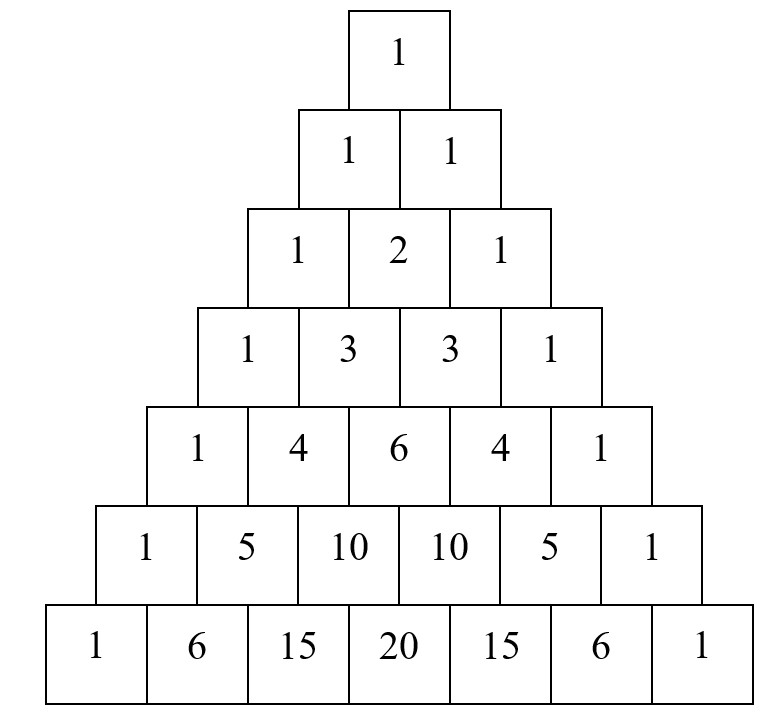
\includegraphics[scale = .39]{pascal1.jpg}
	\end{align}
	\begin{parts}
		
		
		\part You can also write pascals triangle as a table, using this prove pascals identity in figure 3.
		
		\begin{align}
		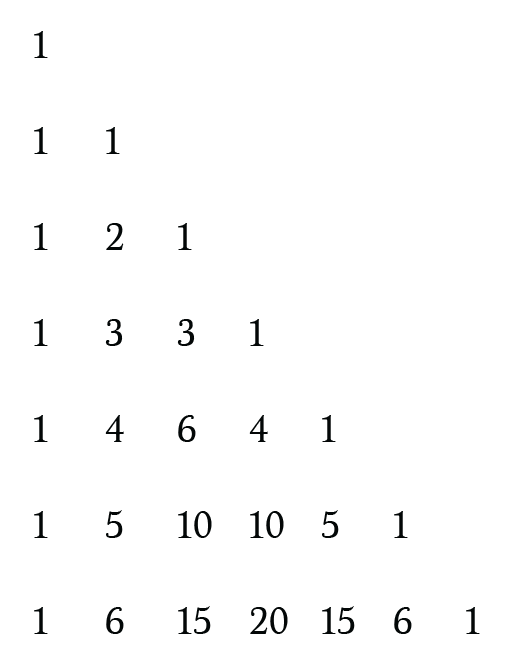
\includegraphics[scale = .2]{pascaltable.png}
		\end{align}
		\begin{align}
		\binom{n}{k} = \binom{n-1}{k-1} + \binom{n-1}{k}
		\end{align}
		
		
		\part We can also look at pascals triangle in the form of a graph. We can observe that the highlighted paths end at the 4 node because there are 4 different paths to reach it. 
		
		\begin{align}
		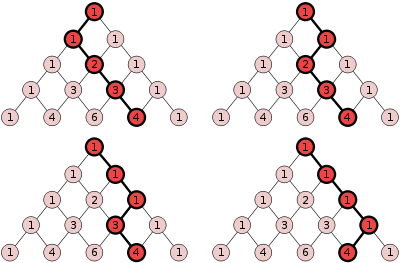
\includegraphics[scale = .5]{pascalgraph.png}
		\end{align}
		
		Now let's look the following expansion.
		\begin{align}
		(x+y)^4 = x^4 + 4x^3y + 6x^2y^2 + 4xy^3 + y^4
		\end{align}
		
		Hopefully by now you should have seen the similarities between the expansion and pascals triangle. This is formally known as Binomial Theorem.
		
		\begin{align}
		(x+y)^n = \sum_{k=0}^{n} \binom{n}{k} x^{n-k}y^{k}
		\end{align}
		
		Give a mathematical proof or explain why the Binomial Theorem is true.
		
		
		
	\end{parts}
	\question
	Asadullah Khan Ghalab has recently discovered the \href{https://en.wikipedia.org/wiki/Fibonacci_number}{Fibonacci series} and the mathematical beauty inherent to it. The Fibonaccis Series is an infinite sequence of integers, starting with $1$ and $2$ and defined recursively after that, for the $n$th term in the array, as $F(n) = F(n-1) + F(n-2)$. Through research on the Fibonacci Series, Ghalib also discovered an interesting set derived from the Fibonacci recurrence.
	
	The \href{http://www.maths.surrey.ac.uk/hosted-sites/R.Knott/Fibonacci/fibGen.html#section6.2}{Wythoff array} is an infinite 2D-array of integers where the $n$th row is formed from the Fibonnaci recurrence using starting numbers $n$ and $\left \lfloor{\phi\cdot (n+1)}\right \rfloor$ where $n \in \mathbb{N}$ and $\phi$ is the \href{https://en.wikipedia.org/wiki/Golden_ratio}{golden ratio} $1.618$ (3 sf).
	
	Ghalib recently studied sets in his discrete math class and needs your help.
	
	\begin{center}
		\begin{tabular}{c c c c c c c c}
			\cellcolor{blue!25}1 & 2 & 3 & 5 & 8 & 13 & 21 & $\cdots$\\
			4 & \cellcolor{blue!25}7 & 11 & 18 & 29 & 47 & 76 & $\cdots$\\
			6 & 10 & \cellcolor{blue!25}16 & 26 & 42 & 68 & 110 & $\cdots$\\
			9 & 15 & 24 & \cellcolor{blue!25}39 & 63 & 102 & 165 & $\cdots$ \\
			12 & 20 & 32 & 52 & \cellcolor{blue!25}84 & 136 & 220 & $\cdots$ \\
			14 & 23 & 37 & 60 & 97 & \cellcolor{blue!25}157 & 254 & $\cdots$\\
			17 & 28 & 45 & 73 & 118 & 191 & \cellcolor{blue!25}309 & $\cdots$\\
			$\vdots$ & $\vdots$ & $\vdots$ & $\vdots$ & $\vdots$ & $\vdots$ & $\vdots$ & \color{blue}$\ddots$\\
		\end{tabular}
	\end{center}
	\begin{parts}
		\part Ghalib is curious whether the Fibonacci series is countable. Prove that it is.
		
		
		\part Ghalib wants you to consider the Modified Wythoff as any array derived from the original, where each entry of the leading diagonal (marked in blue) of the original 2D-Array is replaced with an integer that does not occur in that row. Prove to Ghalib that the Modified Wythoff Array is countable. 
		
		
	\end{parts}
	
	\question After being disappointed with the ``impressive" performance of his students, the discrete mathematics professor at the GradesDontDefineYou University
	cancels his weekly lecture and decides to talk to the students about their recent performance instead. Each student responds differently
	citing different reasons for their supposedly bad performance. 
	There are over 100 students taking this course, of those only 76 responses are deemed \textbf{not invalid} by the professor.
	The Professor saves those responses in a sheet, assigning each of these 76 responses a unique index between 0 and 149,
	inclusive. The invalid responses are simply discarded. Show that \textbf{at least two responses} have indices that are consecutive integers.
\end{questions}


%%%%%%%%%%%%%%%%%%%%%%%%%%%%%%%%%%%%%%%%%%%%%%%%%%%%%%%%%%%%%%%
%%%%%%%%%%%%%%%%%%%%%%%%%%%%%%%%%%%%%%%%%%%%%%%%%%%%%%%%%%%%%%%
%%%%%%%%%%%%%%%%%%%%%%%%%%%%%%%%%%%%%%%%%%%%%%%%%%%%%%%%%%%%%%%
%%%%%%%%%%%%%%%%%%%%%%%%%%%%%%%%%%%%%%%%%%%%%%%%%%%%%%%%%%%%%%%
%%%%%%%%%%%%%%%%%%%%%%%%%%%%%%%%%%%%%%%%%%%%%%%%%%%%%%%%%%%%%%%
%%%%%%%%%%%%%%%%%%%%%%%%%%%%%%%%%%%%%%%%%%%%%%%%%%%%%%%%%%%%%%%


\pagebreak

\section{\Huge Solutions}
\subsection{\huge Sets and Functions}

	
	
\begin{questions}
	
\question

\begin{parts}
	\part ($A \cup B) \cap C$
	\part $\bar A \cup C$
	\part $\overline {(A \cup B)} \cap C$
	\part $(A \cup B \cup C) - ((A \cup B) \cap C) $
\end{parts}
	
	
\question


	% Write your solution here
\begin{parts}
	\part $A \times B$ is defined as $\{(a,b) | a \in A \wedge b \in B\}$. $B \times A$ is defined as $\{(b,a) | b \in B \wedge a \in A\}$. But we know that $(a,b) \neq (b,a)$ unless $a = b$. Therefore $A \times B \neq B \times A$ unless $A = B$.
	\part
	To Prove equality, we will prove $(A \cup B) \cap C \subseteq (A \cap C) \cup (B \cap C)$ and $(A \cap C) \cup (B \cap C) \subseteq (A \cup B) \cap C$ \\
	Considering Left Hand Side
	\[ x \in (A \cup B) \cap C \]
	\[ x \in (A \cup B) \wedge x \in C \]
	\[ (x \in A \vee x \in B) \wedge x \in C \]
	\[ (x \in A \wedge x \in C) \vee (x \in B \wedge x \in C) \]
	\[ x \in (A \cap C) \wedge x \in (B \cap C) \]
	\[ x \in ((A \cap C) \cup (B \cap C)) \]
	Considering Right Hand Side
	\[ x \in ((A \cap C) \cup (B \cap C))\]
	\[ x \in (A \cap C) \vee x \in (B \cap C) \]
	\[ (x \in A \wedge x \in C) \vee (x \in B \wedge x \in C)\]
	\[ (x \in A \vee x \in B) \wedge (x \in C) \]
	\[ (x \in A \cup B) \wedge (x \in C) \]
	\[ x \in ((A \cup B) \cap C) \]
	\[ Q.E.D \]
	\part
	\begin{subparts}
		\subpart By definition, $\mathcal{P}(A)$ is the set of all subsets that can be generated from A, if A and B generate the exact same collection of valid subsets, then it must be that A and B contain the same elements and are therefore equal
		\subpart This part can also be proved by proving it's contrapositive i.e $A \neq B \rightarrow \mathcal{P}(A) \neq \mathcal{P}(B)$. $\mathcal{P}(A)$ is defined as the set of all the possible subsets of A. If A and B are not equal, their sets of all the possible subsets will also not be equal.
		\[ Q.E.D \]
	\end{subparts}
	\part Considering Right Hand Side
	\[ x \in ((A \cap B) \cup (A \cap \bar B)) \]
	\[ x \in (A \cap B) \vee x \in (A \cap \bar B) \]
	\[ (x \in A \wedge x \in B) \vee (x \in A \wedge x \in \bar B) \]
	\[ x \in A \wedge (x \in B \vee x \in \bar B) \]
	\[ x \in A \wedge (x \in B \vee x \notin B) \]
	\[ x \in A\]
	Considering Left Hand Side \\
	We have to proof that $A \subseteq (A \cap B) \cup (A \cap \bar B)$
	We can proof this by proving it's contrapositive. i.e
	\[ \forall x ( ( x \notin ((A \cap B) \cup (A \cap \bar B)) \rightarrow x \notin A) \]
	\[ x \notin ((A \cap B) \cup (A \cap \bar B)) \]
	\[ \neg (x \in ((A \cap B) \cup (A \cap \bar B))) \]
	\[ \neg (x \in ((A \cap B) \vee x \in (A \cap \bar B))) \]
	\[ \neg (x \in (A \cap B)) \wedge \neg (x \in (A \cap \bar B))\]
	\[ \neg (x \in A \wedge x \in B)) \wedge \neg (x \in A \wedge x \in \bar B))\]
	\[ (\neg x \in A \vee \neg x \in B)) \wedge (\neg x \in A \vee \neg (x \in \bar B))\]
	\[ ( x \notin A \vee x \notin B) \wedge (x \notin A \vee (x \in B)\]
	\[ ( x \notin A) \vee (x \notin B \wedge x \in B)\]
	\[ x \notin A \]
	Hence Proved that both sides are subsets of each other and are equal. 
\end{parts}

\question

Possible solutions:
\begin{subparts}
	\subpart Consider the contrapositive: $A \not = B \rightarrow A \times C \not = B \times C$.
	
	Consider sets $A, B$ such that $A \not= B$. Then there exists some $x \in A \cap \bar B$ or its mirror $y \in \bar A \cap B$. Without loss of generality, suppose that x exists. Then $(x,-) \in (A \cap \bar B) \times C$ exists. If $(x,-) \in (A \cap \bar B) \times C$, then $(x,-) \in A \times C$ and $(x,-) \not \in B \times C$. Since $A \times C$ and $B \times C$ differ over $x$, $A \times C \not = B \times C$. Q.E.D.
	
	\subpart We set up a correspondence between sets $A \times C$ and $B \times C$ such that $\forall p \in A \times C, q \in B \times C$ (p maps to q iff $p = q$). We know this correspondence is injective because there is no p which does not correspond to a twin member q. This result follows directly from the assumption that $A \times C = B \times C$. Furthermore, this correspondence is surjective because it is injective and $|A \times C| = |B \times C|$. 
	
	The one-to-one correspondence $\forall p,q$ (p maps to q iff $p = q$) could be elaborated as $\forall a,b$ ($(a, -)$ maps to $(b, -)$ iff $(a,-) = (b,-)$), where $a \in A, b \in B$. Since $(a, -) = (b, -)$ for all elements in the respective sets (as per the definition of the Cartesian Product), $a = b$ for all a and b. Therefore $A = B$. Q.E.D.
	
	
	
\end{subparts}

\question


% Write your solution here
If we just write out what the sum means, we see that parts of successive terms cancel, leaving only two terms: 
\begin{center}
	$\sum_{j = 1}^{n} (a_j - a_{j-1}) = a_1-a_0+a_2-a_1+a_3-a_2+...+a_{n-1}-a_{n-2}+a_n-a_{n-1} = a_n - a_0 $
\end{center}

\question

Here, g(x) takes in something from $\mathbb{Z}$ and then outputs something in $\mathbb{Q}$. Then, f(g(x)) takes in g(x), which is from $\mathbb{Q}$, and outputs something in $\mathbb{R}$. Therefore, for h(x):\\ 
Domain: $\mathbb{Z}$ \\
Co-domain: $\mathbb{R}$ \\
However, to figure out the range we need to combine the two functions: \
\[h(x) = sin(\frac{2x}{3})\]
Range: $\texttt{[-1,1]}$

\question

\begin{parts}
\part
f is \textbf{injective}:
\subsubsection*{Proof:}
Injunction can formally be written as, \[\forall a,b (f(a) = f(b) \implies a = b)\] 
Using our function we can write this as:
\[\forall a,b (a^3 + 20 = b^3 + 20 \implies a = b)\]
\[\equiv \forall a,b (a^3 = b^3 \implies a = b)\]
\[\equiv \forall a,b (a = b \implies a = b)\]
\[\equiv \forall a,b (\bold{T})\]
\[\equiv \bold{T} \qquad \blacksquare\]

\part
f is \textbf{not surjective}:
The answer to this should be easy to see. We just need to find one out of many counter examples to prove that f is not surjective. \\
Surjection is formally written as:
\[\forall y \exists x (f(x) = y) \]
In order to disprove this we need to find a particular y $\in \mathbb{Z}$ such that f(x) $\neq$ y for all x $\in \mathbb{Z}$ \\ 1 is one such value, that is, 
\[ f(x) \neq 1 \qquad \forall x \in \mathbb{Z} \qquad \]

Therefore f is not surjective. $\blacksquare$\\ \\
Refer to page 145 of your course book for more on how to prove/disprove injunction and/or surjection.

\part
f is \textbf{not bijective}:\\ \\
A necessary condition for f to be bijective is that it has to be surjective. Since f is not surjective therefore it is not bijective. $\blacksquare$



\end{parts}	
\end{questions}	

%%%%%%%%%%%%%%%%%%%%%%%%%%%%%%%%%%%%%%%%%%%%%%%%%%%%%%%%%%%%%%%
%%%%%%%%%%%%%%%%%%%%%%%%%%%%%%%%%%%%%%%%%%%%%%%%%%%%%%%%%%%%%%%
\subsection{\huge Counting and Sequences}

\begin{questions}
	\question
	
	
		% Write your solution here
	\begin{parts}
		\part Base Case:- For n = 1, 
		\[(2(1) - 1)^2 = \frac{1}{3}(1)(2(1) - 1)(2(1) + 1)\]
		\[(1)^2 = \frac{1}{3}(1)(1)(3)\]
		\[1 = 1\]
		Inductive Step:- We assume that 
		\[ \sum_{i = 1}^{k} (2i -1 )^2 = \frac{1}{3}k(2k - 1)(2k + 1)\]
		To Prove:-
		\[ \sum_{i = 1}^{k+1} (2i -1 )^2 = \frac{1}{3}(k+1)(2(k+1) - 1)(2(k+1) + 1) = \frac{1}{3}(k+1)(2k+1)(2k+3)\]
		\[ \sum_{i = 1}^{k+1} (2i -1 )^2 \]
		\[ \sum_{i = 1}^{k} (2i -1 )^2  + (2(k+1) - 1)^2\]
		\[ \frac{1}{3}k(2k - 1)(2k + 1) + (2k+1)^2\]
		\[ \frac{1}{3}(2k + 1)(k(2k - 1) + 3(2k+1))\]
		\[ \frac{1}{3}(2k + 1)(2k^2 + 5k +3)\]
		\[ \frac{1}{3}(2k + 1)(k + 1)(2k +3)\]
		\[ Q.E.D. \]
		\part Base Case:- For n = 1,
		\[ 1(1+2) = \frac{1}{6}(1)(1+1)(2(1)+7) \]
		\[ 3 = \frac{1}{6}(2)(9) \]
		\[ 3 = 3 \]
		Inductive Step:- We assume that 
		\[ \sum_{i = 1}^{k} i(i+2) = \frac{1}{6}k(k+1)(2k+7) \]
		To Prove:- 
		\[ \sum_{i = 1}^{k+1} i(i+2) = \frac{1}{6}(k+1)(k+2)(2k+9) \]
		\[ \sum_{i = 1}^{k+1} i(i+2) \]
		\[ \sum_{i = 1}^{k} i(i+2) + (k+1)(k+3) \]
		\[ \frac{1}{6}k(k+1)(2k+7) + (k+1)(k+3) \]
		\[ \frac{1}{6}(k+1)(k(2k+7) + 6(k+3)) \]
		\[ \frac{1}{6}(k+1)(2k^2 + 15k + 18) \]
		\[ \frac{1}{6}(k+1)(k+2)(2k + 9) \]
		\[ Q.E.D. \]
		
		%part 3
		\part Base Case:- For n = 1,
		\[  \frac{1}{1(1+1)} = \frac{1}{1+1} \]
		\[  \frac{1}{2} = \frac{1}{2} \]
		Inductive Step:- We assume that 
		\[ \sum_{i = 1}^{k} \frac{1}{i(i+1)} = \frac{k}{k+1} \]
		To Prove:- 
		\[ \sum_{i = 1}^{k+1} \frac{1}{i(i+1)} = \frac{k+1}{k+2} \]
		\[ \sum_{i = 1}^{k+1} \frac{1}{i(i+1)} \]
		\[ \sum_{i = 1}^{k} \frac{1}{i(i+1)} + \frac{1}{(k+1)(k+2)} \]
		\[ \frac{k}{k+1} + \frac{1}{(k+1)(k+2)} \]
		\[ \frac{k(k+2) + 1}{(k+1)(k+2)} \]
		\[ \frac{k^2 + 2k + 1}{(k+1)(k+2)} \]
		\[ \frac{(k+1)^2}{(k+1)(k+2)} \]
		\[ \frac{(k+1)}{(k+2)} \]
		\[ Q.E.D. \]
		
		%part 4
		\part Base Case:- For n = 1,
		\[ 1(2^1) = 2^{1+1}(1-1) + 2 \]
		\[ 2 = 2^{2}(0) + 2 \]
		\[ 2 = 2 \]
		Inductive Step:- We assume that 
		\[ \sum_{i = 1}^{k} i(2^i) = 2^{k+1}(k-1) + 2 \]
		To Prove:- 
		\[ \sum_{i = 1}^{k+1} i(2^i) = 2^{k+2}(k) + 2 \]
		\[ \sum_{i = 1}^{k+1} i(2^i)\]
		\[ \sum_{i = 1}^{k} i(2^i) + (k+1)(2^{k+1})\]
		\[ 2^{k+1}(k-1) + 2 + (k+1)(2^{k+1})\]
		\[ 2^{k+1}((k-1) + (k+1)) + 2 \]
		\[ 2^{k+1}(2k) + 2 \]
		\[ 2^{k+2}(k) + 2 \]
		\[ Q.E.D. \]
		
		%part 5
		\part Base Case:- For n = 1,
		\[ 1(1!) = (1+1)! - 1 \]
		\[ 1 = 2 - 1 \]
		\[ 1 = 1 \]
		Inductive Step:- We assume that 
		\[ \sum_{i = 1}^{k} i(i!) = (k+1)! - 1 \]
		To Prove:- 
		\[ \sum_{i = 1}^{k + 1} i(i!) = (k+2)! - 1 \]
		\[ \sum_{i = 1}^{k + 1} i(i!)\]
		\[ \sum_{i = 1}^{k} i(i!) + (k+1)((k+1)!)\]
		\[ (k+1)! - 1 + (k+1)((k+1)!)\]
		\[ (k+1)!(1 + (k+1)) - 1 \]
		\[ (k+1)!(k+2) - 1 \]
		\[ (k+2)(k+1)! - 1 \]
		\[ (k+2)! - 1 \]
		\[ Q.E.D. \]
	\end{parts}

	
	\question

	
	
	% Write your solution here
	\begin{parts}
		\part Since the arrangement has to be taken in consideration for roommate-sock combinations, the possibilities would be: $\Perm{10}{5}= 30,240.$
		\part Since the colour is disregarded over here and it does not matter if the same colour combination is repeated by different individuals, the possibilities would be: $\Comb{10}{5}= 252$
		\part The colours mentioned are one specific combination (red, teal, orange, pink and magenta) out of a total of $\Comb{10}{5}$ so the probability of this combination occurring is reduced to: $\frac{\Comb{5}{5}}{\Comb{10}{5}}=\frac{1}{252}$
		\part Since one roommate hoards 3 pairs of socks, there are 7 remaining sock pairs to share from for the other 4 friends. Now he has two distinct possibilities: Either to choose from his own 3 pairs (one’s he has hoarded) or one from the other 7 pairs that his friends are sharing. This would make the final permutation: $\Perm{3}{1} \times \Perm{7}{4} + \Perm{7}{5} = 5040$
		\part Now since there is a restriction introduced - the hoarder is not allowed to wear the other colors of socks. This eliminates his choice and he can only wear from the ones he has hoarded. The new permutation is: $\Perm{3}{1} \times \Perm{7}{4} = 2520$
		\part Again, in this situation only colour combinations are considered. For this, the arrangement can be overlooked. The complete combination of the colours the hoarder could possibly wear from his collection of 3 pairs and the other friends from their 7 pairs is: $\Comb{3}{1} \times \Comb{7}{4} = 105$
	\end{parts}
	
	%Question 3 Rayyan, a) Combination with repetition, b) double counting c) simple pigeon hole principle
	\question
	%write your question here


	\begin{parts}
		\part We model this situation as distributing $n$ apples among $m$ children, where we add an extra condition that all of them must receive at least one apple. Disregarding the condition, the question is a simple combination with repetition problem so how can we incorporate the condition. Instead of trying to distribute $n$ apples among $m$ children we say we will give one apple to each child then find the number of way of distribute the remaining apples among the children. There fore the number of apples left handing $m$ apples, one to each child, will be $n - m$ and the number of ways to distribute these among $m$ children, applying the following formula of combination with repetition
		$$\binom{(n) + (r) - 1}{(r) - 1}$$
		we have
		$$\binom{(n-m)+(m)-1}{(m)-1}$$
		$$\binom{n-1}{m-1}$$
		\part To count the above in a different way we say that we will hand the first child $k$ apples where k cannot be less than 1 and cannot be greater than $n - m - 1$ because at least one apple needs be to handed to other $m-1$ children. For each value of $k$ there will be a certain number of ways to distribute the $n-k$ remaining apples among the $m -1$ children. Following the same strategy as before and handing one apple to each of the $m-1$ children we are left with $n-k-m+1$ apples to be distributed among $m-1$ children, applying combination with repetition
		$$\binom{(n-k-m+1)+(m-1)-1}{(m-1)-1}$$
		$$\binom{n - k-1}{m-2}$$
		From here we can say that if we sum the number of ways to distribute the remaining apples over all possible values of $k$ it will be the same as the number ways of distributing $n$ apples among $m$ children where each gets at least one and hence,
		$$\binom{n-1}{m-1} = \sum_{k=1}^{n-m+1}\binom{n-k-1}{m-2}$$
		\part The first thing to note is that all $b_i$ will be different since they belong to a set. Secondly none of them will have a value less than one that is the least value any element can possibly have is one. The number of possible subsets that $S$ can have is equal to $2^m$ since it has $m$ elements and excluding the empty subset it is $2^m-1$. Now the largest subset will be equal to $S$ itself and have sum $n$ that is the maximum sum any subset can have will be $n$ and the minimum sum a subset can have is $1$. Thus the total possible values of the sum of a subset can range from $1$ to $n$ that is the sum of a subset can take $n$ possible values and we have $2^m-1$ non-empty subsets. From the question we know $2^m-1>n$ thus by the pigeon hole principle there must be at least two subsets which have the same sum. When we have two such sets we can just remove the common elements in them and we will have two non empty disjoint subsets that have the same sum.
	\end{parts}

	
	
	\question
	Prove the following
	
	\begin{parts}
		\part
		Simple substitution. 
		$$\frac{n!}{k!(n-k)!} = \frac{n!}{(n-k)!(n-(n-k))!}$$
		
		$$\frac{n!}{k!(n-k)!} = \frac{n!}{(n-k)!k!}$$
		
		NOTE: This also shows symmetry in each row of Pascal's triangle. 
		
		\part
		$$\sum_{i=1}^{n} i =\binom{n+1}{2} $$
		
		$$\frac{n^2 + n}{2} =\binom{n+1}{2} $$
		
		$$\frac{n^2 + n}{2} = \frac{(n+1)!}{2!(n+1)-2)!}$$
		
		$$\frac{n^2 + n}{2} = \frac{(n+1)!}{2!(n+1)-2)!}$$
		
		$$\frac{n^2 + n}{2} = \frac{(n+1)n!}{2!(n-1)!}$$
		
		Using: $(n-1)! = \frac{n!}{n}$
		
		$$\frac{n^2 + n}{2} = \frac{(n+1)n!}{2!\frac{n!}{n}!}$$
		
		$$\frac{n^2 + n}{2} = \frac{(n+1)n}{2!}$$
		
		$$\frac{n^2 + n}{2} = \frac{n^2 + n}{2}$$
		
		\part
		
		First we can expand the sum.
		
		$$ \binom{n}{0} + \binom{n}{1} + \binom{n}{2} + \cdots + \binom{n}{n} = 2^n$$
		
		We can intemperate this a little differently. 
		
		We think of each choose function being summed as the number of ways to choose $k$ thing from a set of cardinality $n$.
		
		For example from $S = \{1,2,3\}$
		
		Ways to can choose 0 thing = 1. $\{\}$
		
		Ways to can choose 1 thing = 3. $\{\{1\},\{2\},\{3\}\}$
		
		Ways to can choose 2 thing = 3. $\{\{1,2\},\{2,3\},\{3,1\}\}$
		
		Ways to can choose 3 thing = 1. $\{\{1,2,3\}\}$
		
		Numerically this looks like.
		
		$$ \binom{3}{0} + \binom{3}{1} + \binom{3}{2} + \binom{3}{3} = 2^3$$
		
		$$ 1 + 3 + 3 + 1 = 8$$
		
		By counting number of ways to choose $0-n$ things from a set of size $n$, essentially we are counting the cardinality of the powerset.
		
	\end{parts}
	
	
	\question


	\begin{parts}
		\part  We can say the columns are the $k$ value and the rows are the $n$ value. 
		From looking at the table we can realize the recursive relation. That the value of the current node is the sum the one above and to the left $\binom{n-1}{k-1}$ and one above $\binom{n-1}{k}$. This is just a formal representation of how most people derive Pascal's triangle by hand.
		
		\part
		If we expand a binomial we write it as.
		
		$$(x+y)^4 = (x+y)(x+y)(x+y)(x+y)$$
		
		Conventionally we would expand this algebraically, however we can view the expansion with combinatorics. If we where to multiply this out(FOIL), it would the same as asking how many different ways can you choose $x^ny^k$ where $n+k=4$ for $n$'s and $k$'s. NOTE: the 4 in $n+k=4$ corresponds to the fourth row of Pascals Triangle.
		
		We can see if $n=4,k=0$, there is only one way to choose this and that is where from each parenthesis the $x$ is chosen a multiplied.  
		
		$$(x+y)^4 = (x_1+y_1)(x_2+y_2)(x_3+y_3)(x_4+y_4)$$
		
		$$x^4 = x_1x_2x_3x_4$$
		
		Another example is where $n=1,k=3$, there is 4 ways to choose this through.
		
		$$(x+y)^4 = (x_1+y_1)(x_2+y_2)(x_3+y_3)(x_4+y_4)$$
		
		$$xy^3 = x_1y_2y_3y_4$$
		$$xy^3 = y_1x_2y_3y_4$$
		$$xy^3 = y_1y_2x_3y_4$$
		$$xy^3 = y_1y_2y_3x_4$$
		
		Now we can connect this Pascals Triangle in graph form. We can think that moving left corresponds with choosing a $x$ and moving right corresponds with a $y$. From the graph we can see the four different ways to 4 node in the fourth row.
		
		$$left, right, right, right$$
		$$right, left, right, right$$
		$$right, right, left, right$$
		$$right, right, right, left$$
	\end{parts}



	\question




	\begin{parts}

		\part
		% Write your solution here
		If we create a function f(x) where $ x \in \mathbb{Z^+}$,
		\[ f(x)=
		\begin{cases} 
		1 &  \textrm{if x=1}\\
		2 & \textrm{if x=2}  \\
		f(x-1)+f(x-2) & \textrm{x$>$2} 
		\end{cases}
		\]
		Through this function, we can see that all positive integers are being mapped to the Fibonacci series. Since each integer maps to a unique element in the Fibonacci, the function is injective. Since each element in the Fibonacci is being mapped from a unique integer, the function is surjective therefore the function is bijective and since we have proved a bijection from the set of positive integers to the Fibonacci series, we have proved that the Fibonacci series is countable.
	
	
		\part
		% Write your solution here
		Every row in the Wythoff array is a Fibonnaci sequence. As we have proved in part (a) that the Fibonacci series is countable, every row of the Wythoff is countable, as every row is a modified Fibonacci series. If we replace each leading diagonal in each row, we will be replacing each with a number not present in the row, meaning every element in the row will be a unique number. Because of this, each modified row will still remain countable and bijective with $\mathbb{Z^+}$
		
		If we take the cartesian product of $\mathbb{Z^+}$, $\mathbb{Z^+} \times \mathbb{Z^+}$, we can see each tuple in $\mathbb{Z^+} \times \mathbb{Z^+}$ as (a,b). a can be seen as the row number and b can be seen as the column number. With this we can establish a bijection between $\mathbb{Z^+} \times \mathbb{Z^+}$ and the Wythoff array similiar to how we did it in part (a). As each element of the Wythoff array has a different column number and row number, their is a surjection between $\mathbb{Z^+} \times \mathbb{Z^+}$ and the Wythoff. As we have already established that each row will have no repeating elements, if an element does repeat in the Wythoff, it will be in a different column and hence will be related to a different tuple of $\mathbb{Z^+} \times \mathbb{Z^+}$, thus establishing an injection. As we have established both and injection and surjection, we can say that the Wythoff array is bijective with \textbf{$\mathbb{Z^+} \times \mathbb{Z^+}$}. As $\mathbb{Z^+}$ is countable, $\mathbb{Z^+} \times \mathbb{Z^+}$ is also countable and since we have established a bijection between the Wythoff and $\mathbb{Z^+} \times \mathbb{Z^+}$, we can safely say that the wythoff is countable.
	
		
	\end{parts}
	
\end{questions}

\end{document}